\documentclass[tikz,border=10pt]{standalone}
\usetikzlibrary{arrows.meta, positioning}

\tikzset{
    block/.style={rectangle, draw, minimum width=3cm, minimum height=1cm, text centered},
    line/.style={draw, thick, -Stealth}
}

\begin{document}
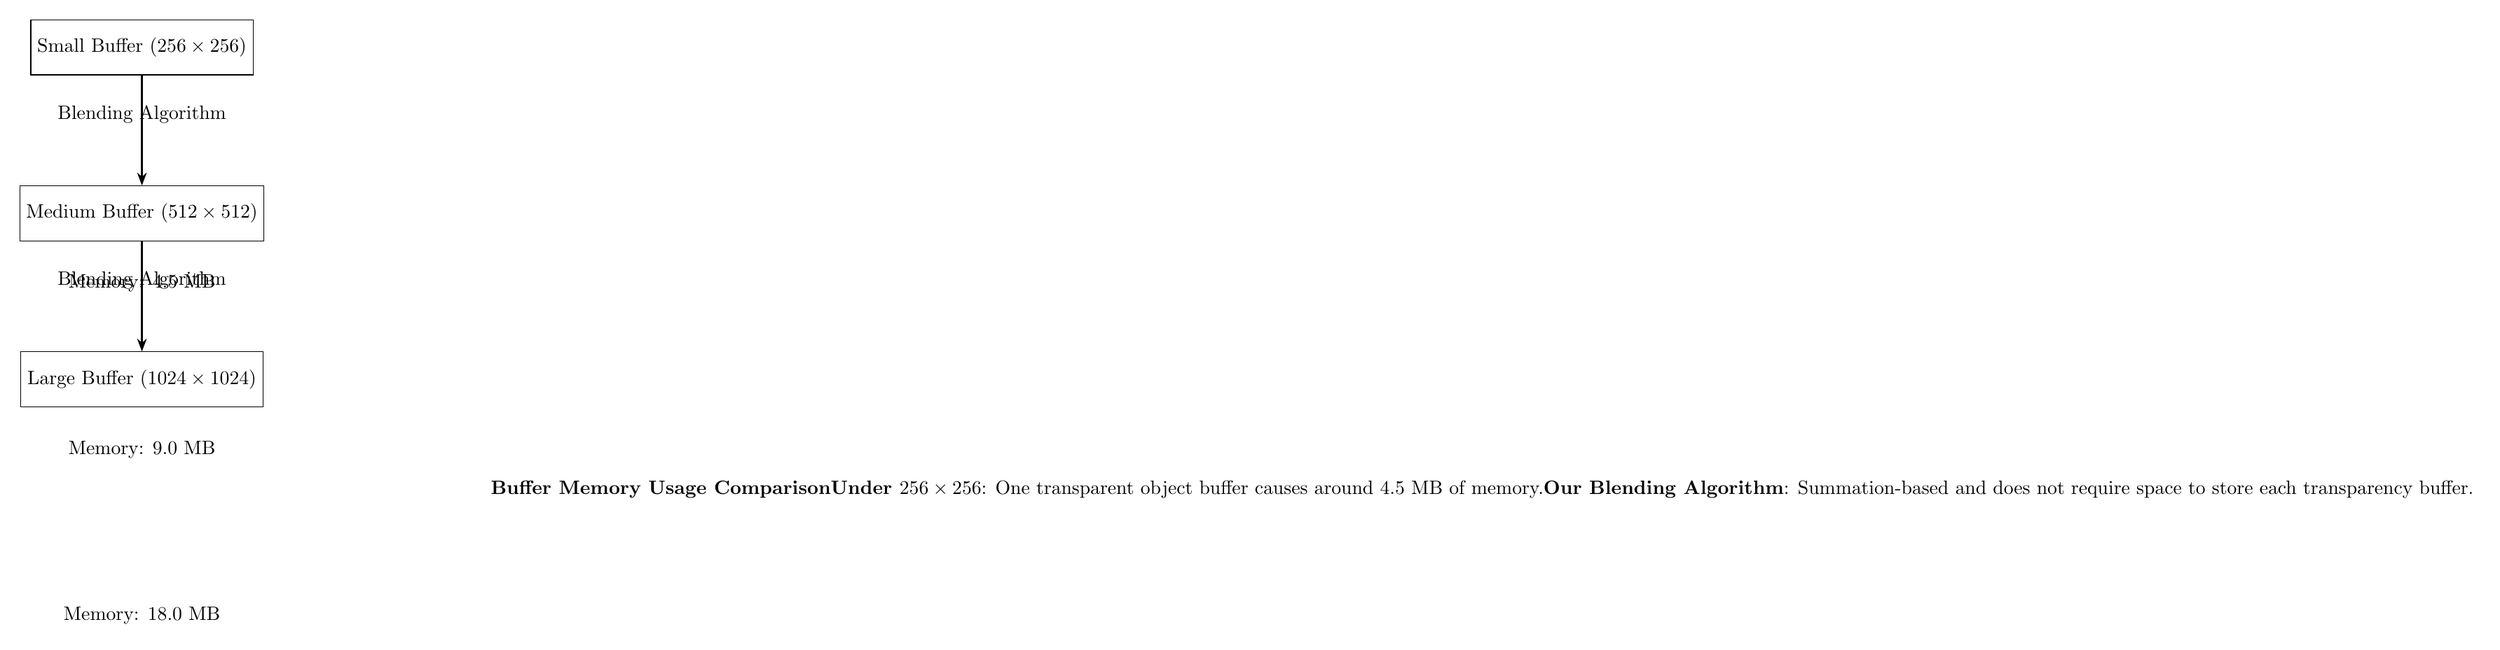
\begin{tikzpicture}[node distance=2cm]
    % Nodes
    \node (small_buffer) [block] {Small Buffer (\(256 \times 256\))};
    \node (medium_buffer) [block, below=of small_buffer] {Medium Buffer (\(512 \times 512\))};
    \node (large_buffer) [block, below=of medium_buffer] {Large Buffer (\(1024 \times 1024\))};

    % Memory Usage Labels
    \node (memory_small) [below=of small_buffer, yshift=-1.5cm] {Memory: 4.5 MB};
    \node (memory_medium) [below=of medium_buffer, yshift=-1.5cm] {Memory: 9.0 MB};
    \node (memory_large) [below=of large_buffer, yshift=-1.5cm] {Memory: 18.0 MB};

    % Lines connecting nodes
    \draw [line] (small_buffer) -- node[above] {Blending Algorithm} (medium_buffer);
    \draw [line] (medium_buffer) -- node[above] {Blending Algorithm} (large_buffer);

    % Explanation Text
    \node (explanation) [right=of large_buffer, xshift=2cm, yshift=-2cm] {
        \textbf{Buffer Memory Usage Comparison} \\
        \textbf{Under \(256 \times 256\)}: One transparent object buffer causes around 4.5 MB of memory. \\
        \textbf{Our Blending Algorithm}: Summation-based and does not require space to store each transparency buffer.
    };
\end{tikzpicture}
\end{document}